\documentclass[12pt]{article}

\usepackage{sbc-template}
\usepackage{graphicx,url}
\usepackage[utf8]{inputenc}
\usepackage[brazil]{babel}
\usepackage{float}
     
\sloppy

\title{Projeto e Desenvolvimento de uma \textit{Dataglove} de Baixo Custo para Aplicações em Realidade Virtual}

\author{Rabah Zeineddine}


\address{Faculdade de Computação e informática -- Universidade Presbiteriana Mackenzie
  \\
  São Paulo, SP -- Brasil
  \email{rabah.zeineddine@gmail.com}
}

\begin{document} 

\maketitle

\begin{abstract}
    Abstract
\end{abstract}
     
\begin{resumo} 
    Resumo
\end{resumo}


\section{Introdução}

Com o avanço da tecnologia e para tornar cada vez mais preciso e mais próximo da realidade a interação humano-computador surge a necessidade de novos dispositivos e hardwares mais potentes que ajudam a melhorar essa interação capturando e analisando cada vez mais dados precisos em tempo real. \textit{Dataglove} ou luva de dados, é uma luva fabricada com tecnologias altas que permite capturar os gestos e os movimentos da mão do ser humano e transmitir esses dados para um computador por exemplo. Com a ajuda de softwares desenvolvidos especificamente para este tipo de aplicação, os dados capturados podem ser simulados para apresentar alguns tipos de aplicações como a aplicação do movimento da mão dentro da Realidade Virtual.

Hardwares pequenos de alta funcionalidade já estão disponíveis para o uso como a placa Arduíno. O Arduíno é um dispositivo relativamente pequeno de placa única que pode ser usado para objetos interativos independentes. Junto ao Arduíno existe uma série de sensores e dispositivos plugáveis compatíveis com a placa para estender a sua capacidade e poder cada vez mais fazer projetos mais complexos e completos. Uma placa típica de Arduíno é composta por um controlador, algumas linhas de entrada e saída digital e analógica além da interface serial ou USB. A interação entre a placa e o computador por exemplo é feita através de alguns softwares desenvolvidos utilizando diferentes linguagens de programação.

Dentro deste contexto, este projeto apresenta os conceitos básicos de uma luva de dados e algumas aplicações dessa luva no mundo real como também uma comparação dos preços das luvas atuais. Além da apresentação da luva, são apresentados os conceitos da placa Arduíno e alguns modelos existentes, especificamente é apresentado a placa Arduíno \textit{LilyPad} com seus detalhes e especificações, além da utilização da plataforma Unity3D para simular os dados capturados da luva.

Com esta placa de micro controlador, o projeto propõe o desenvolvimento de uma luva de dados de baixo custo utilizando a placa de Arduíno \textit{LilyPad} junto a alguns sensores externos para a captura de dados utilizando a plataforma Unity3D para a modulação e a simulação dos dados.


\section{Referencial teórico} \label{sec:fundamentosDatagloves}

Esta seção apresenta os conceitos básicos da \textit{dataglove} mostrando algumas aplicações na Realidade Virtual.

\subsection{Conceitos básicos da \textit{Datagloves}}

A \textit{Dataglove} ou também conhecida como \textit{cyberglove} é um dispositivo de entrada de dados para a interação humano-computador fabricado no formato de uma luva vestível que captura o movimento da mão utilizando vários sensores tecnológicos \cite{buscher_2012}

\begin{figure}[H]
    \centering
    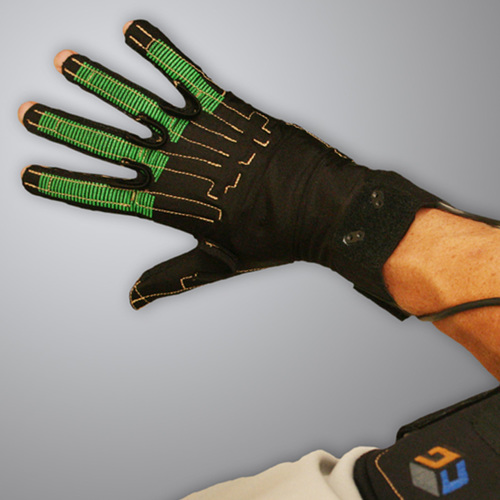
\includegraphics[width=.7\textwidth]{images/cg3-thumb.jpeg}
    \caption{\textit{Cyberglove III}}
    \label{fig:cyberglove3-1}
\end{figure}

A mão de ser humano, especificamente, é uma maneira geral das pessoas interagirem com o ambiente real. Os gestos da mão é uma parte muito importante do corpo do ser humano a serem capturados e simulados num mundo virtual, assim poderá ter um controle mais preciso e mais próximo para a realidade usando uma simulação da mão capturada em mundo real e aplicada em mundo virtual como na Realidade Virtual ou Realidade Aumentada \cite{linn_2017}

\subsection{Exemplos da \textit{Datagloves}}

Há vários modelos da datagloves que já foram desenvolvidos com o objetivo de capturar os gestos e os movimentos da mão do ser humano e transmitir os dados capturados para o computador. Um exemplo deles, mostrado na figura \ref{fig:cyberglove3-2}, é a \textit{CyberGlove III}.

\begin{figure}[H]
    \centering
    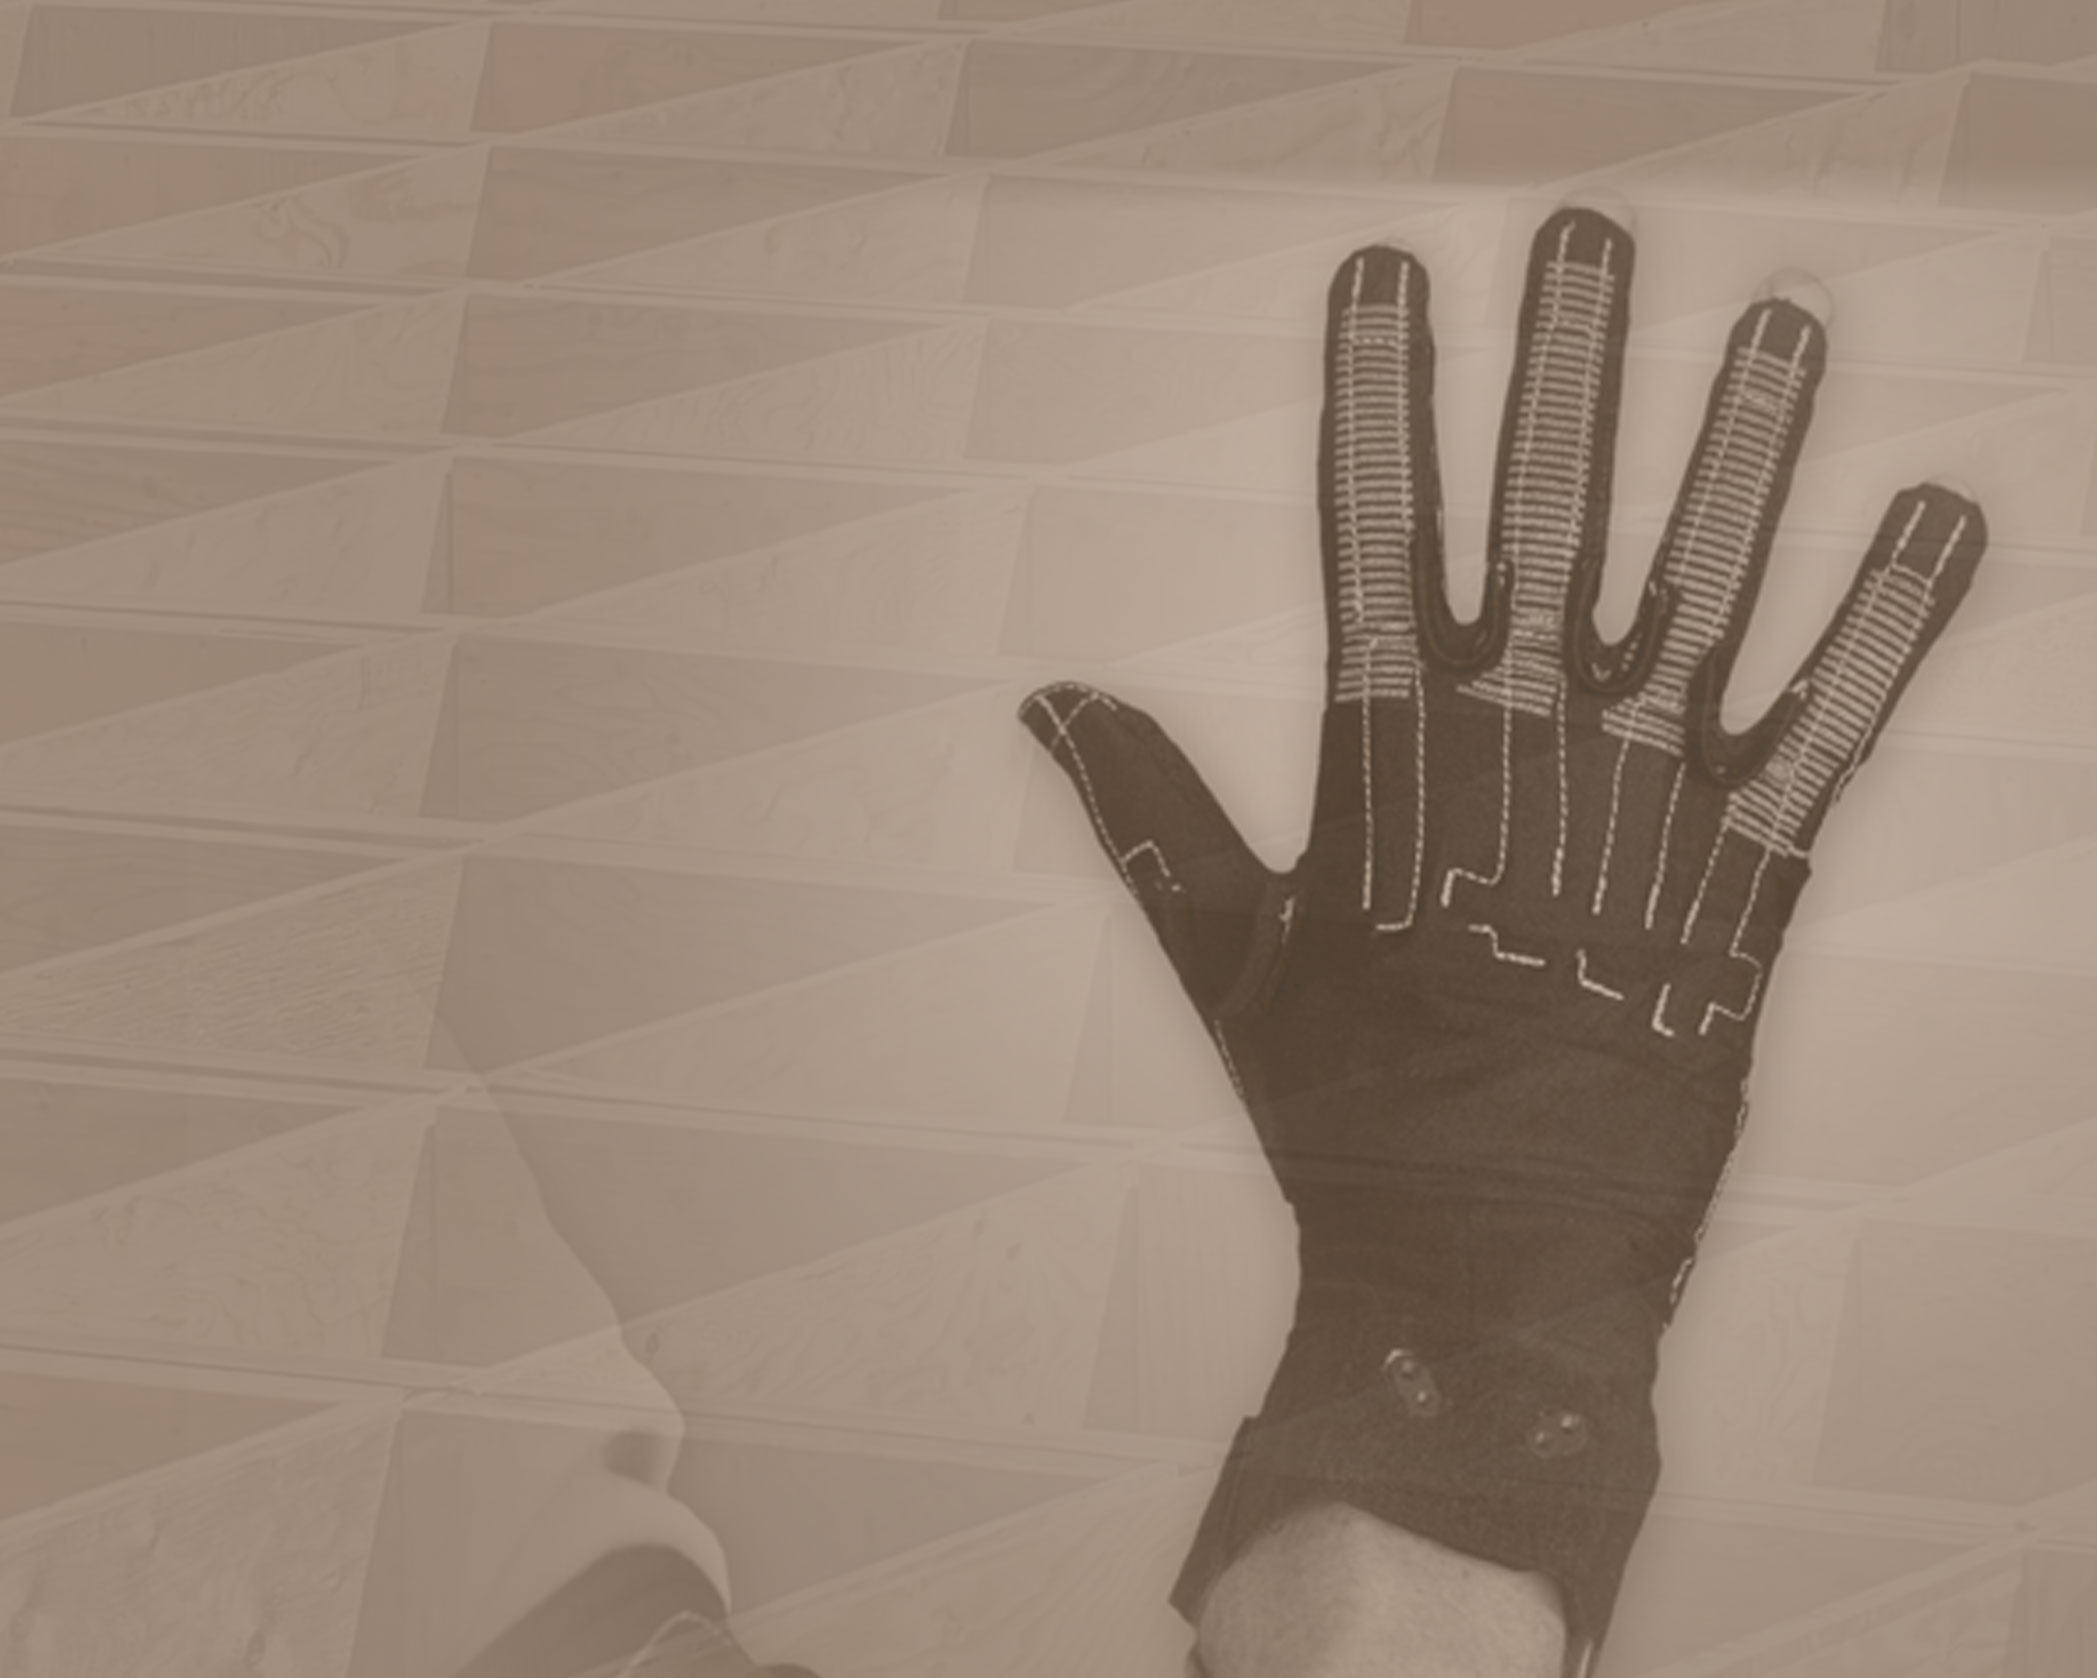
\includegraphics[width=.7\textwidth]{images/cyberglove-iii-2.jpg}
    \caption{\textit{Cyberglove III}}
    \label{fig:cyberglove3-2}
\end{figure}

A \textit{Cyberglove} III possui até 22 sensores como também possui a tecnologia de transmissão de dados pelo wifi 802.11g, além disso a bateria dele dura 2 horas e captura por volta de 100 registro/seg , ele possibilita a captura dos gestos da mão e a transmissão com umas tecnologias bem avançadas \cite{mardiyanto_2017}
\\ \\ Um outro exemplo da dataglove, mostrado na figura \ref{fig:hw_data_glove_wireless_01}, é a 5DT:

\begin{figure}[H]
    \centering
    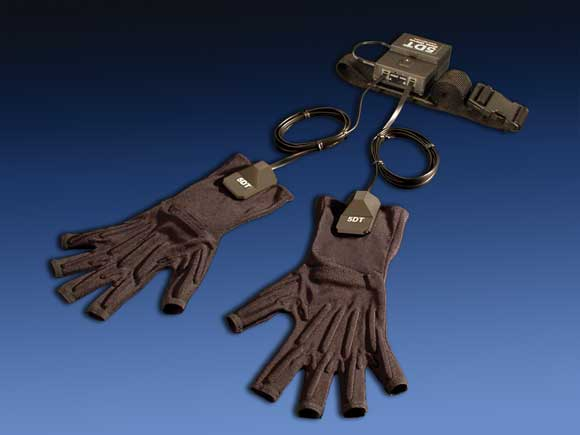
\includegraphics[width=.7\textwidth]{images/hw_data_glove_wireless_01.jpg}
    \caption{\textit{Dataglove 5DT}}
    \label{fig:hw_data_glove_wireless_01}
\end{figure}

A luva 5DT foi desenhada para satisfazer os requisitos modernos da captura de dados e animação profissional, oferecendo conforto, facilidade de uso. Interage com um computador via USB ou via WIFI, tendo 14 sensores para detecção do movimento da mão como também a bateria dura até 8 horas \cite{o-larnnithipong_2016}
\\ \\
Existe também um outro conceito no modo de utilização de uma luva de dados ou dataglove, a \textit{CyberGrasp} por exemplo, mostrado na figura \ref{fig:grasp3}, é um sistema de luva de inovação de retorno de força para os dedos e a mão, ou seja, a \textit{CyberGrasp} permita que você sinta alguns objetos 3D gerados pelo computador em um mundo virtual, conforme mostrado na figura \ref{fig:grasp3}

\begin{figure}[H]
    \centering
    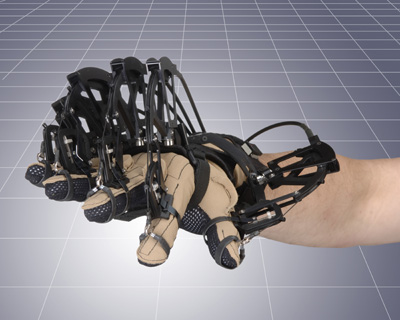
\includegraphics[width=.7\textwidth]{images/grasp3.jpg}
    \caption{\textit{CyberGrasp}}
    \label{fig:grasp3}
\end{figure}

A \textit{CyberGrasp} acrescenta alguns resistores nos dedos a mais em comparação com a \textit{CyberGlove III} para poder controlar a mão do ser humano \cite{o-larnnithipong_2016}

\subsection{Aplicações de \textit{DataGloves} em Realidade Virtual}

Os sistemas da Realidade Virtual dependem dos dispositivos de entrada de captura de dados de ambientes no mundo real e transmitir informações adquiridas para um ambiente virtual. Este é um processo importante para providenciar o melhor sentimento dentro de um ambiente virtual. Os gestos e os movimentos do ser humano são os dados mais capturados com os dispositivos de entrada de dados da Realidade Virtual \cite{hee_2017}
\\ \\ 
A dataglove é um dos dispositivos utilizado para captura de gestos da mão como mostra a figura \ref{fig:ManusVR}

\begin{figure}[H]
    \centering
    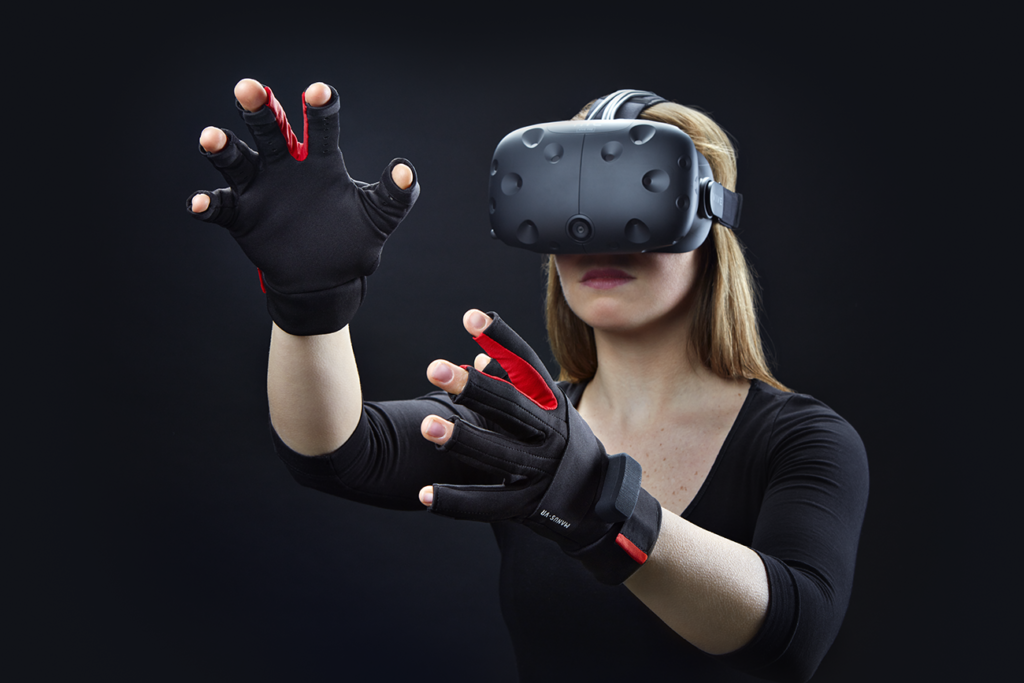
\includegraphics[width=.7\textwidth]{images/ManusVR_Glove_moodfoto2-1024x683.png}
    \caption{\textit{Dataglove utilizado na realidade virtual.}}
    \label{fig:ManusVR}
\end{figure}

A aplicação da dataglove na Realidade Virtual ajuda bastante no nível de precisão de captura dos gestos e movimentos da mão do ser humano, os dados são capturados no tempo real e transmitidos para um computador através de USB ou WIFI e esses dados recebidos passarão por um software em que faz a simulação desses dados capturados para produzir um modelo de uma mão virtual dentro do ambiente virtual \cite{Tham_2018}

\begin{figure}[H]
    \centering
    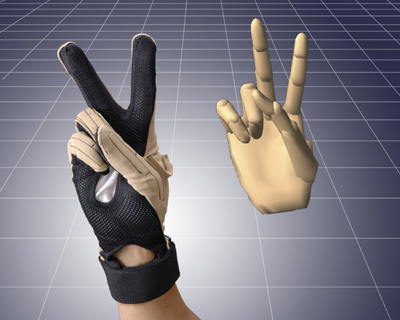
\includegraphics[width=.7\textwidth]{images/cyberglove2.jpg}
    \caption{\textit{Simulação de CyberGlove II}}
    \label{fig:cyberglove2}
\end{figure}

A figura \ref{fig:cyberglove2} mostra um modelo computacional utilizando \textit{CyberGlove II} como dispositivo de captura de gestos onde dá pra perceber que a mão foi modulada perfeitamente e esse modelo pode ser utilizado dentro do mundo virtual.

\subsection{Comparação de Preços de \textit{Datagloves}}

As \textit{datagloves} existentes no mercado e alguns representados acima, tem um preço alto que varia entre 500 \$ e chega até 5,495 \$,  ou seja,  um preço bem elevado para ser disponível para qualquer pessoa. A figura \ref{fig:pricing} mostra alguns preços de alguns dataglove 5DTs:

\begin{figure}[H]
    \centering
    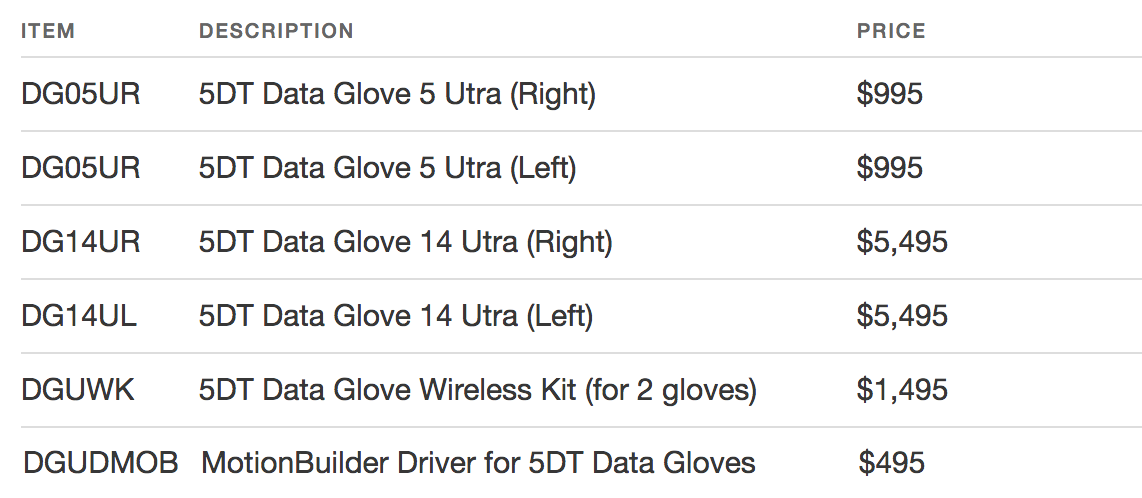
\includegraphics[width=.7\textwidth]{images/pricing.png}
    \caption{\textit{5DT CyberGlove Pricing}}
    \label{fig:pricing}
\end{figure}

O preço da luva varia depende de vários aspectos, a quantidade de sensores como a qualidade deles, o material utilizado na fabricação da luva como também alguns dispositivos de WiFI e Bluetooth que podem ser utilizados para a transmissão de dados \cite{Pereira_2013}

\subsection{Arduíno}

Arduíno é uma plataforma eletrônica aberta baseada na facilidade de uso de hardware e de software. As placas de Arduíno são capazes de ler entradas como luz de sensores, botões entre outros e transformar isso em uma saída de dados, ou seja , em dados capturados transformados em dados computacionais.\\
\\A figura \ref{fig:arduinoUno} mostra uma placa de Arduíno UNO:

\begin{figure}[H]
    \centering
    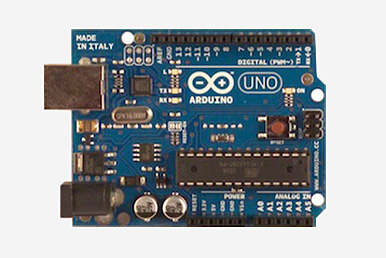
\includegraphics[width=.7\textwidth]{images/ArduinoUnoFront240.jpg}
    \caption{\textit{Arduíno UNO USB}}
    \label{fig:arduinoUno}
\end{figure}

A ideia atrás de desenvolvimento do Arduíno é disponibilizar uma plataforma para providenciar um hardware de desenvolvimento aberto para criar dispositivos e projetos integrando vários tipos de sensores e dispositivos plugáveis compatíveis com ele.  Após o crescimento do Arduíno no mercado, vários dispositivos foram fabricados para servir algum proposito especifico, como \textit{Wireless}, sensores, \textit{Bluetooth} entre outros.  Arduíno tem a facilidade de aprender linguagem e bibliotecas baseadas em C++ como também um IDE para a própria interface de programação. Arduíno é considerado como plataforma de hardware independentes que pode operar nos sistemas operacionais Windows, Linux ou MAC.

\subsection{\textit{LilyPad}}

Há vários modelos de placas de Arduínos fabricadas até o momento, como Arduíno Uno, Arduíno Duemilanove, Arduíno Diecimila e várias outras placas com especificações diferentes de capacidade e compatibilidade de hardware. O LilyPad \cite{Buechley_2008} é um tipo de placa de Arduíno que foi desenhada para tecnologias têxteis e projetos vestíveis de tamanho pequeno.
\\ \\A figura \ref{fig:lilypad} mostra uma placa Arduíno LilyPad:
\begin{figure}[H]
    \centering
    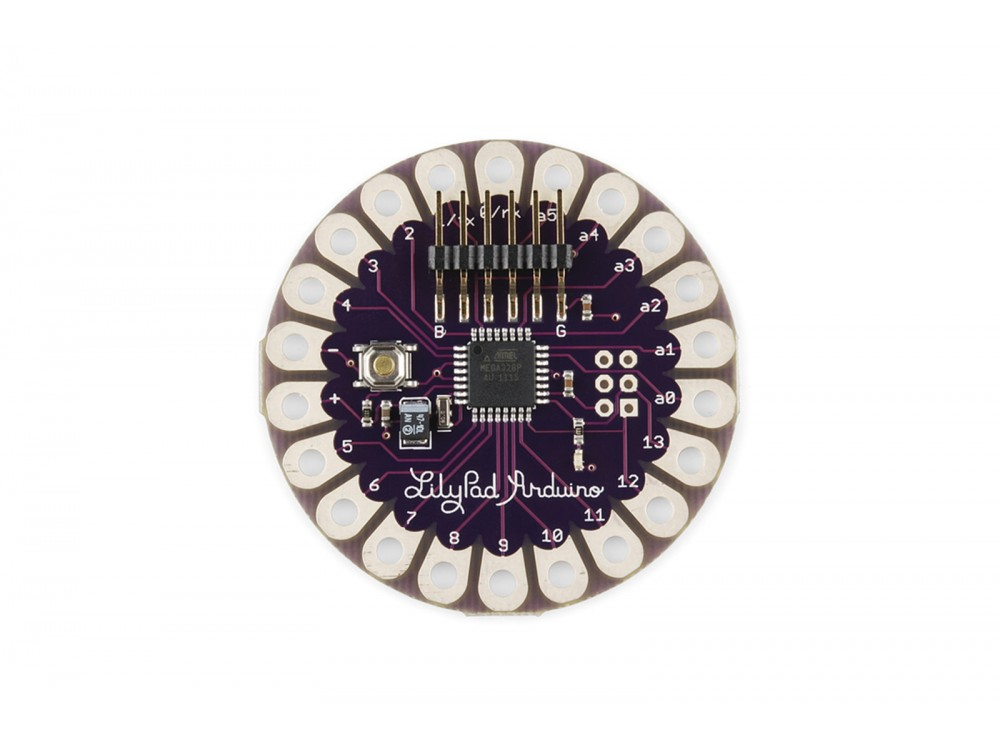
\includegraphics[width=.7\textwidth]{images/lilypad_img.jpg}
    \caption{\textit{Arduíno Lilypad}}
    \label{fig:lilypad}
\end{figure}


A placa de Arduíno LilyPad é baseada em ATmega168V, uma versão de baixo consumo de energia de ATmega168 ou ATmega328V. ATmega168 é um micro controlador AVR baseado na arquitetura RISC de 8-bit. ATmega168 combina com 16KB ISP memoria Flash com a capacidade de ler-enquanto-escreve, 512B EEPROM, 1KB SRAM, 23 linhas de entrada e saída, 32 registradores entre outras especificações técnicas.  Com todas as especificações do LilyPad, ele apresenta um alto desempenho como também um consumo muito baixo de energia.  Uma placa de Arduíno com um tamanho pequeno igual LilyPad e com um desempenho razoavelmente alto, pode ser utilizada em projetos vestíveis e robóticos como uma luva de dados e outros projetos que necessitam uma placa pequena onde pode ser portátil e oculta.

\bibliographystyle{sbc}
\bibliography{sbc-template}

\end{document}